\documentclass{report}
\usepackage[utf8]{inputenc}
\usepackage[T1]{fontenc}
\usepackage{CormorantGaramond}
\usepackage{fontspec}
\usepackage{geometry}
\usepackage[table]{xcolor}
\usepackage{tabularx}
\usepackage{graphicx}
\usepackage{mathtools}
\usepackage[bottom]{footmisc}
\usepackage[italian]{babel}
\usepackage{hyperref}
\usepackage{titlesec}
\usepackage{listings}
\usepackage{color}
\usepackage{graphicx}
\usepackage{fancyhdr}
\usepackage{xltabular}

\renewcommand{\headrulewidth}{0.4pt}
\renewcommand{\footrulewidth}{0.4pt}

\lstset{ % General setup for the package
    basicstyle=\small\sffamily,
    numbers=left,
     numberstyle=\tiny,
    frame=tb,
    tabsize=4,
    columns=fixed,
    showstringspaces=false,
    showtabs=false,
    keepspaces,
    commentstyle=\color{red},
    keywordstyle=\color{blue}
}

\geometry{
a4paper,
total = {170mm, 240mm},
left = 20mm,
top = 20mm,
}

\setlength{\headheight}{33.60004pt}

\setlength{\parindent}{0em}
\setlength{\parskip}{0.7em}

\titlespacing*{\section}{0pt}{0.7em}{0.5em}
\titlespacing*{\subsection}{0pt}{0.7em}{0.5em}

\newcommand{\gassets}{../}




\renewcommand{\title}{
    Piano di qualifica

    \tiny Versione documento: \textit{V1.0.8}
}

\newcommand{\people}{
    \normalsize
    \begin{center}
        \begin{tabularx}{7cm}{l | X}            
            \textbf{Uso} & Esterno\\
            \textbf{Destinatario} & Committente\\
            & Cliente \\
        \end{tabularx}
    \end{center}
}

\fancypagestyle{plain}{%
    \fancyhead{} % clear all header fields
    \fancyhead[L]{\leftmark}
    \fancyhead[R]{\textit{SWEasabi} \includegraphics[height=30pt]{\gassets global-assets/img/loghi/SWEasabi_compact_logo.png}}
    \fancyfoot{} % clear all footer fields
    \fancyfoot[L]{\thepage}
    \fancyfoot[R]{Piano di qualifica}
}

\begin{document}

\pagestyle{fancy}

\fancyhead{} % clear all header fields
\fancyhead[L]{\leftmark}
\fancyhead[R]{\textit{SWEasabi} \includegraphics[height=30pt]{\gassets global-assets/img/loghi/SWEasabi_compact_logo.png}}
\fancyfoot{} % clear all footer fields
\fancyfoot[L]{\thepage}
\fancyfoot[R]{Piano di qualifica}


\input{\gassets global-assets/tex/header}
\thispagestyle{empty}
\clearpage
\pagenumbering{Roman}
\section*{Registro delle modifiche}

\newcommand{\pzerozerouno}{
    \begin{center}
        \begin{tabularx}{\linewidth}{l | X}            
            \textbf{Approvazione} & \\
            \hline
            \textbf{Redazione} & Mattia Casarotto\\
            \hline
            \textbf{Verifica} & Luca Pierobon\\
        \end{tabularx}
    \end{center}
}

\newcommand{\vzerozerouno}{
    \hline
    0.0.1 & \textbf{data} & 
        \begin{itemize}
            \item Aggiunta sezione "Qualità di processo".
        \end{itemize}
    
    & \pzerozerouno\\
}
\newcommand{\pzerozerodue}{
    \begin{center}
        \begin{tabularx}{\linewidth}{l | X}            
            \textbf{Approvazione} & Massarenti Alessandro\\
            \hline
            \textbf{Redazione} & Casarotto Mattia\\
            \hline
            \textbf{Verifica} & Pierobon Luca \\
        \end{tabularx}
    \end{center}
}

\newcommand{\mzerozerodue}{
    \begin{itemize}
        \item Aggiunta sezione "Introduzione"
    \end{itemize}
}

\newcommand{\vzerozerodue}{
    \hline
    0.0.2 & 5 mar 2023 & \mzerozerodue & \pzerozerodue\\
}
\newcommand{\pzerozerotre}{
    \begin{center}
        \begin{tabularx}{\linewidth}{l | X}            
            \textbf{Approvazione} & Alessandro Massarenti\\
            \hline
            \textbf{Redazione} & Luca Pierobon\\
            \hline
            \textbf{Verifica} & Luca Pierobon\\
        \end{tabularx}
    \end{center}
}

\newcommand{\mzerozerotre}{
    \begin{itemize}
        \item Aggiunto registro modifiche
    \end{itemize}
}

\newcommand{\vzerozerotre}{
    \hline
    0.0.3 & 6 mar 2023 & \mzerozerotre & \pzerozerotre\\
}
\newcommand{\pzerounozero}{
    \begin{center}
        \begin{tabularx}{\linewidth}{l | X}            
            \textbf{Verifica} & Pierobon Luca \\
        \end{tabularx}
    \end{center}
}

\newcommand{\mzerounozero}{
    \begin{itemize}
        \item Revisione del documento
    \end{itemize}
}

\newcommand{\vzerounozero}{
    \hline
    0.1.0 & 7 mar 2023 & \mzerounozero & \pzerounozero\\
}
\newcommand{\pzerounouno}{
    \begin{center}
        \begin{tabularx}{\linewidth}{l | X}            
            \textbf{Approvazione} & Alessandro Massarenti\\
            \hline
            \textbf{Redazione} & Michele Bonavigo\\
            \hline
            \textbf{Verifica} & Luca Pierobon\\
        \end{tabularx}
    \end{center}
}

\newcommand{\mzerounouno}{
    \begin{itemize}
        \item Aggiunta sezione "Specifica dei test"
    \end{itemize}
}

\newcommand{\vzerounouno}{
    \hline
    0.1.1 & 15 mar 2023 & \mzerounouno & \pzerounouno\\
}
\newcommand{\pzerounodue}{
    \begin{center}
        \begin{tabularx}{\linewidth}{l | X}            
            \textbf{Approvazione} & Massarenti Alessandro \\
            \hline
            \textbf{Redazione} & Casarotto Mattia \\
            \hline
            \textbf{Verifica} & Bonavigo Michele \\
            & Massarenti Alessandro \\
        \end{tabularx}
    \end{center}
}

\newcommand{\mzerounodue}{
    \begin{itemize}
        \item Aggiunta sezione "Valutazioni per l'automiglioramento"
    \end{itemize}
}

\newcommand{\vzerounodue}{
    \hline
    0.1.2 & 15 mar 2023 & \mzerounodue & \pzerounodue\\
}
\newcommand{\pzerounotre}{
    \begin{center}
        \begin{tabularx}{\linewidth}{l | X}            
            \textbf{Approvazione} & Massarenti Alessandro \\
            \hline
            \textbf{Redazione} & Zarantonello Giorgio \\
            \hline
            \textbf{Verifica} & Pierobon Luca \\
            & Casarotto Mattia \\
        \end{tabularx}
    \end{center}
}

\newcommand{\mzerounotre}{
    \begin{itemize}
        \item Aggiunta sezione "Qualità di prodotto"
    \end{itemize}
}

\newcommand{\vzerounotre}{
    \hline
    0.1.3 & 19 mar 2023 & \mzerounotre & \pzerounotre\\
}
\newcommand{\pzeroduezero}{
    \begin{center}
        \begin{tabularx}{\linewidth}{l | X}            
            \textbf{Verifica} & Pierobon Luca \\
        \end{tabularx}
    \end{center}
}

\newcommand{\mzeroduezero}{
    \begin{itemize}
        \item Revisione del documento
    \end{itemize}
}

\newcommand{\vzeroduezero}{
    \hline
    0.2.0 & 19 mar 2023 & \mzeroduezero & \pzeroduezero\\
}
\newcommand{\pzerodueuno}{
    \begin{center}
        \begin{tabularx}{\linewidth}{l | X}            
            \textbf{Approvazione} & Luca Pierobon\\
            \hline
            \textbf{Redazione} & Giorgio Zarantonello\\
            \hline
            \textbf{Verifica} & Michele Bonavigo\\
        \end{tabularx}
    \end{center}
}

\newcommand{\mzerodueuno}{
    \begin{itemize}
        \item Aggiunta sezione "Resoconto delle attività di verifica"
    \end{itemize}
}

\newcommand{\vzerodueuno}{
    \hline
    0.2.1 & 19 mar 2023 & \mzerodueuno & \pzerodueuno\\
}
\newcommand{\pzerotrezero}{
    \begin{center}
        \begin{tabularx}{\linewidth}{l | X}            
            \textbf{Verifica} & Michele Bonavigo\\
            & Luca Pierobon\\
            & Alessandro Massarenti\\
        \end{tabularx}
    \end{center}
}

\newcommand{\mzerotrezero}{
    \begin{itemize}
        \item Revisione del documento
    \end{itemize}
}

\newcommand{\vzerotrezero}{
    \hline
    0.3.0 & 31 mar 2023 & \mzerotrezero & \pzerotrezero\\
}
\newcommand{\punozerozero}{
    \begin{center}
        \begin{tabularx}{\linewidth}{l | X}            
            \textbf{Approvazione} & Pierobon Luca\\
        \end{tabularx}
    \end{center}
}

\newcommand{\munozerozero}{
    \begin{itemize}
        \item Approvata versione 1.0.0
    \end{itemize}
}

\newcommand{\vunozerozero}{
    \hline
    1.0.0 & 2 apr 2023 & \munozerozero & \punozerozero\\
}
\newcommand{\punozerouno}{
    \begin{center}
        \begin{tabularx}{\linewidth}{l | X}            
            \textbf{Approvazione} & Pierobon Luca \\
            \hline
            \textbf{Redazione} & Bonavigo Michele \\
            \hline
            \textbf{Verifica} & Casarotto Mattia \\
        \end{tabularx}
    \end{center}
}

\newcommand{\munozerouno}{
    \begin{itemize}
        \item Eliminato glossario dal documento
        \item Corretti nomi registo modifiche
    \end{itemize}
}

\newcommand{\vunozerouno}{
    \hline
    1.0.1 & 2 apr 2023 & \munozerouno & \punozerouno\\
}
\newcommand{\punozerodue}{
    \begin{center}
        \begin{tabularx}{\linewidth}{l | X}            
            \textbf{Approvazione} & Romano Davide\\
            \hline
            \textbf{Redazione} & Zarantonello Giorgio\\
            \hline
            \textbf{Verifica} & Peron Samuel\\
        \end{tabularx}
    \end{center}
}

\newcommand{\munozerodue}{
    \begin{itemize}
        \item Rimosso registro modifiche dall'indice
    \end{itemize}
}

\newcommand{\vunozerodue}{
    \hline
    1.0.2 & 31 lug 2023 & \munozerodue & \punozerodue\\
}
\newcommand{\punozerotre}{
    \begin{center}
        \begin{tabularx}{\linewidth}{l | X}            
            \textbf{Approvazione} & Romano Davide\\
            \hline
            \textbf{Redazione} & Zarantonello Giorgio\\
            \hline
            \textbf{Verifica} & Peron Samuel\\
        \end{tabularx}
    \end{center}
}

\newcommand{\munozerotre}{
    \begin{itemize}
        \item Aggiunta lista iniziale dei test di unità
        \item Aggiunta lista dei test di sistema
    \end{itemize}
}

\newcommand{\vunozerotre}{
    \hline
    1.0.3 & 01 ago 2023 & \munozerotre & \punozerotre\\
}
\newcommand{\punozeroquattro}{
    \begin{center}
        \begin{tabularx}{\linewidth}{l | X}            
            \textbf{Approvazione} & Romano Davide\\
            \hline
            \textbf{Redazione} & Zarantonello Giorgio\\
            \hline
            \textbf{Verifica} & Peron Samuel\\
        \end{tabularx}
    \end{center}
}

\newcommand{\munozeroquattro}{
    \begin{itemize}
        \item Aggiunta lista dei test di integrazione
    \end{itemize}
}

\newcommand{\vunozeroquattro}{
    \hline
    1.0.4 & 07 ago 2023 & \munozeroquattro & \punozeroquattro\\
}

%Tabella
\begin{center}
    \begin{xltabular}{\linewidth}{|l|l|X|X|}            
        \hline
        \textbf{Versione} & \textbf{Data} & \textbf{Modifica}& \textbf{Persone}\\
        \vunozeroquattro
        \vunozerotre
        \vunozerodue
        \vunozerouno
        \vunozerozero
        \vzerotrezero
        \vzerodueuno
        \vzeroduezero
        \vzerounotre
        \vzerounodue
        \vzerounouno
        \vzerounozero
        \vzerozerotre
        \vzerozerodue
        \vzerozerouno
        \hline

    \end{xltabular}
\end{center}

\tableofcontents
\clearpage
\pagenumbering{arabic}
\chapter{Introduzione}
\section{Scopo del documento}
Lo scopo di questo documento è quello di presentare in modo ordinato e scorrevole gli standard di qualità del gruppo, basandosi su caratteristiche misurabili tramite metriche oggettive. Questi standard verranno implementati con l'obiettivo di conseguire un miglioramento continuo attraverso azioni correttive, e non semplicemente come misurazioni statiche. All'interno del documento verranno inoltre dettagliati test e attività di verifica utilizzate per rilevare la qualità descritta.

Le metriche di qualità si possono individuare tramite le seguenti sigle: \textbf{M - Sigla - Numero}

dove le diverse parti indicano:

\begin{itemize}
    \item \textbf{M} indica che si tratta di una metrica;
    \item \textbf{Sigla} si riferisce alla tipologia di metrica, in particolare:
    \begin{itemize}
        \item \textbf{PD} indica prodotto;
        \item \textbf{PC} indica processo;
        \item \textbf{T} indica test.
    \end{itemize}
    \item \textbf{Numero} è il numero identificativo della metrica, a partire da 01.
\end{itemize}

\section{Scopo del prodotto}
Il risparmio delle risorse del Pianeta e in particolare delle fonti energetiche è entrato con forza nell'agenda politica dell’Unione Europea. Fra gli impatti più evidenti, spicca la crescita esponenziale del prezzo del gas, risorsa ancora largamente utilizzata come materia prima per la produzione di energia elettrica.
Per far fronte al rincaro delle bollette energetiche, molti comuni italiani stanno annunciando tagli sull’illuminazione pubblica, che necessita di una quantità considerevole di energia elettrica.

Il capitolato C2, \textit{Lumos Minima}, pone come obiettivo lo sviluppo di un sistema per l'ottimizzazione dell'illuminazazione pubblica che permetta ai gestori di sfruttare la possibilità di regolare l'intensità della luce emessa dagli impianti di illuminazione.

\section{Glossario}
Un glossario utile con alcune definizioni per lavorare al progetto al fine di chiarire eventuali termini che possono generare dubbi interpretativi:

\section{Maturità del documento}
Il presente documento è redatto con un approccio incrementale in modo tale da trattare modifiche o aggiunte in modo efficiente. Non può pertanto essere considerato definitivo nella sua attuale versione.

\section{Riferimenti e richiami}
\subsection{Riferimenti normativi}
\begin{itemize}
    \item Capitolato d'appalto C2 - Lumos Minima: \\ \url{https://www.math.unipd.it/~tullio/IS-1/2022/Progetto/C2.pdf}
\end{itemize}

\subsection{Riferimenti informativi}
\begin{itemize}
    \item Slide T02 del corso di Ingegneria del Software: \\ \url{https://www.math.unipd.it/~tullio/IS-1/2022/Dispense/T02.pdf}
    \item Slide T12 del corso di Ingegneria del Software: \\ \url{https://www.math.unipd.it/~tullio/IS-1/2022/Dispense/T12.pdf}
    \item Metriche di Progetto: \\ \url{https://it.wikipedia.org/wiki/Metriche_di_progetto}
    \item Software Metrics: \\ \url{https://en.wikipedia.org/wiki/Software_metric}
    \item Indice di Gulpease: \\ \url{https://it.wikipedia.org/wiki/Indice_Gulpease}
\end{itemize}
\chapter{Qualità di processo}\label{qualita-di-processo}

\section{Introduzione}
Lo standard utilizzato per la qualità dei processi è il ISO/IEC 12207:1995, con particolare attenzione ad alcuni processi che verranno esposti di seguito.

\section{Processi primari}
\subsection{Fornitura}
Con processo di fornitura si intende tutte le attività atte a selezionare risorse e procedure necessarie per portare a termine il progetto. 

\textbf{Metriche}
\begin{itemize}
    \item \textbf{MPC01: Budget At Completion}
    \begin{itemize}
        \item \textbf{Spiegazione}: Valore preventivato per la realizzazione del progetto;
        \item \textbf{Metrica di misurazione}: Costo in euro;
        \item \textbf{Valore ottimale}: Valore preventivato;
        \item \textbf{Soglia accettabile}: <= 10\%.
    \end{itemize}
    \item \textbf{MPC02: Budget Variance}
    \begin{itemize}
        \item \textbf{Spiegazione}: Indica se alla data corrente la spesa effettiva è in difetto o in cesso rispetto a quella preventivata;
        \item \textbf{Metrica di misurazione}: Costo in euro, calcolato attraverso la seguente formula: \textbf{BV = BCWS - ACWP}
        \begin{itemize}
            \item \textbf{BV} indica \textbf{B}udget \textbf{V}ariance;
            \item \textbf{BCWS} indica \textbf{B}udgeted \textbf{C}ost of \textbf{W}ork \textbf{S}cheduled, ossia il costo previsto (in euro) per realizzare delle attività alla data corrente;
            \item \textbf{ACWP} indica \textbf{A}ctual \textbf{C}ost of \textbf{W}ork \textbf{P}erformed, ossia il costo effettivo (in euro) della realizzazione delle suddette attività.
        \end{itemize}
        \item \textbf{Valore ottimale}: 0;
        \item \textbf{Soglia accettabile}: <= 10\%.
    \end{itemize}
    \item \textbf{MPC03: Schedule Variance}
    \begin{itemize}
        \item \textbf{Spiegazione}: Indica se il progetto è in linea, in anticipo o in ritardo rispetto alle attese alla data preventivata;
        \item \textbf{Metrica di misurazione}: Giorni, calcolati attraverso la seguente formula: \textbf{SV = BCWP - BCWS}
        \begin{itemize}
            \item \textbf{SV} indica \textbf{S}chedule \textbf{V}ariance;
            \item \textbf{BCWP} indica \textbf{B}udgeted \textbf{C}ost of \textbf{W}ork \textbf{P}erformed indica il valore (in giorni) delle attività realizzata alla data corrente;
            \item \textbf{BCWS} indica \textbf{B}udgeted \textbf{C}ost of \textbf{W}ork \textbf{S}cheduled, ossia il costo previsto (in giorni) per realizzare delle attività alla data corrente;
        \end{itemize}
        \item \textbf{Valore ottimale}: 0;
        \item \textbf{Soglia accettabile}: <= 7 giorni.
    \end{itemize}
\end{itemize}

\subsection{Sviluppo}


\subsubsection{Analisi dei requisiti}


\subsubsection{Design e progettazione}


\subsubsection{Codifica}


\section{Processi di supporto}


\subsection{Documentazione}
\begin{itemize}
    \item \textbf{MPC: Indice di Gulpease}
    \begin{itemize}
        \item \textbf{Spiegazione}: Si tratta di un indice di leggibilità del testo;
        \item \textbf{Metrica di misurazione}: Numero intero, calcolato attraverso la seguente formula: \textbf{$89 + \frac{300*(NF)-10*(NL)}{NP}$};
            \begin{itemize}
                \item \textbf{NF} indica \textbf{N}umero \textbf{F}rasi;
                \item \textbf{NL} indica \textbf{N}umero \textbf{L}ettere;
                \item \textbf{NP} indica \textbf{N}umero \textbf{P}arole;
            \end{itemize}
        \item \textbf{Valore ottimale}: 80-100;
        \item \textbf{Soglia accettabile}: 60-100.
    \end{itemize}
\end{itemize}

\begin{itemize}
    \item \textbf{MPC: Correttezza ortografica}
    \begin{itemize}
        \item \textbf{Spiegazione}: Indica il numero di errori grammaticali presenti nel testo;
        \item \textbf{Metrica di misurazione}: Numero intero;
        \item \textbf{Valore ottimale}: 0;
        \item \textbf{Soglia accettabile}: <= 5\%.
    \end{itemize}
\end{itemize}


\subsection{Validazione}
\chapter{Qualità di prodotto}\label{qualita-di-prodotto}

\section{Introduzione}
Utilizzando lo standard ISO/IEC 12207:1995 , abbiamo individuato le Qualità che si ritengono necessarie durante l'intero ciclo di vita del prodotto, definendo metriche e obiettivi specifici al loro conseguimento

Sono questi riportati di seguito 

\section{Affidabilità}
\begin{itemize}
    \item \textbf{Descrizione}
    \begin{itemize}
        \item L'affidabilità del prodotto si riferisce alla sua capacità di svolgere le sue funzioni , a prescidere dal manifestarsi di errori,provandone ad eliminare la loro incidenza
    \end{itemize}
    
    \item \textbf{metriche}
    \begin{itemize}
        \item MPD01
        \begin{itemize}
            \item \textbf{Spiegazione}: Misurazione dei difetti del prodotto;
        \item \textbf{Metrica di misurazione}: Percentuale;
        \item \textbf{Valore ottimale}: 80\% ;
        \item \textbf{Soglia accettabile}: 60\%.
        \item \textbf{Note}: I valori potranno essere modificati .
        \end{itemize}
    \end{itemize}
    \end{itemize}

\section{Efficienza}
\begin{itemize}
    \item \textbf{Descrizione}
    \begin{itemize}
        \item L'efficienza del prodotto si riferisce alla sua capacità di svolgere le sue funzioni nel minor tempo possibile e utilizzando il minor numero di risorse.
    \end{itemize}
    
    \item \textbf{metriche}
    \begin{itemize}
        \item MPD02
        \begin{itemize}
\item \textbf{Spiegazione}: Tempo medio di risposta;
        \item \textbf{Metrica di misurazione}: Secondi;
        \item \textbf{Valore ottimale}: 5 Secondi;
        \item \textbf{Soglia accettabile}: 7 Secondi.
        \end{itemize}
    \end{itemize}
    \end{itemize}

\section{Funzionalità}
\begin{itemize}
    \item \textbf{Descrizione}
    \begin{itemize}
        \item La Funzionalità del prodotto si riferisce alla capacità del prodotto di svolgere le funzioni previste in modo completo e corretto.
    \end{itemize}
    
    \item \textbf{metriche}
    \begin{itemize}
        \item MPD03
        \begin{itemize}
            \item \textbf{Spiegazione}: Copertura dei requisiti;
        \item \textbf{Metrica di misurazione}: Percentuale;
        \item \textbf{Valore ottimale}: 100\% dei requisiti obbligatori;
        \item \textbf{Soglia accettabile}: 100\% dei requisiti obbligatori.
        \end{itemize}
    \end{itemize}
    \end{itemize}
    
\section{Manutenibilità}
\begin{itemize}
    \item \textbf{Descrizione}
    \begin{itemize}
        \item La Manutenibilità del prodotto si riferisce alla capacità del prodotto di essere modificato e mantenuto in modo efficiente.
    \end{itemize}
    
    \item \textbf{metriche}
    \begin{itemize}
        \item MPD04
        \begin{itemize}
            \item \textbf{Spiegazione}: Comprensibilità del codice;
        \item \textbf{Metrica di misurazione}: Percentuale;
        \item \textbf{Valore ottimale}: 85\% - 100\% ;
        \item \textbf{Soglia accettabile}: 60\% - 100\% .
        \end{itemize}
    \end{itemize}
    \end{itemize}


\section{Portabilità}
\begin{itemize}
    \item \textbf{Descrizione}
    \begin{itemize}
        \item La Portabilità del prodotto si riferisce alla capacità del prodotto di essere utilizzato in diverse piattaforme e ambienti.
    \end{itemize}
    
    \item \textbf{metriche}
    \begin{itemize}
        \item MPD05
        \begin{itemize}
            \item \textbf{Spiegazione}: Compatibilità del prodotto;
        \item \textbf{Metrica di misurazione}: Percentuale;
        \item \textbf{Valore ottimale}: 85\% - 100\% ;
        \item \textbf{Soglia accettabile}: 60\% - 100\% .
        \end{itemize}
    \end{itemize}
    \end{itemize}



\section{Usabilità}

    \begin{itemize}
    \item \textbf{Descrizione}
    \begin{itemize}
    \item L'Usabilità del prodotto si riferisce alla capacità del prodotto di essere utilizzato in modo efficace, efficiente e soddisfacente dagli utenti finali.
    \end{itemize}

    \item MPD06
        \begin{itemize}
            \item \textbf{Spiegazione}: Facilità d'uso del prodotto;
            \item \textbf{Metrica di misurazione}: Numero di errori compiuti dagli utenti durante l'utilizzo del prodotto;
            \item \textbf{Valore ottimale}: Inferiore a 1 errore per utente;
            \item \textbf{Soglia accettabile}: Inferiore a 2 errori per utente.
        \end{itemize}
    \end{itemize}
    

\chapter{Specifica dei test}\label{specifica-dei-test}
L'analisi dinamica consiste nell'esecuzione di vari oggetti di prova allo scopo di studiare il comportamento del programma in un insieme finito di casi rappresentativi di tutte le possibili esecuzioni del codice. Ogni esecuzione rappresenta un test, che possono essere di vario tipo, qui di seguito elencati.
Il gruppo SWEasabi ha deciso che, per perseguire la maggior correttezza del prodotto possibile, l'attività di verifica verrà svolta in parallelo allo sviluppo. L'obiettivo da perseguire sarà quindi quello di rendere i test il più automatici possibile allo scopo di non rallentare il processo di sviluppo.

Inoltre, giudicando prematura la definizione dei test in questa fase, il gruppo ha deciso di definirli nelle successive versioni di questo documento.

\section{Test di unità}
I test di unità hanno come scopo quello di dimostrare la correttezza di ciascuna unità individualmente, arrivando al 100\% quando ogni singola unità è stata testata con esito positivo. 

\section{Test di integrazione}
I test di integrazione verificano l'integrazione tra le componenti software, ovvero che due o più unità già testate con esito positivo lavorino insieme in modo corretto generando il risultato e comportamento atteso.

\section{Test di sistema}
I test di sistema si occupano di verificare il comportamento del sistema, controllando che aderisca correttamente ai requisiti software individuati nell'Analisi dei Requisiti.

\section{Test di accettazione}
I test di accettazione costituiscono il collaudo del prodotto, svolto in presenza del committente, con lo scopo di verificare il soddisfacimento di tutti i requisiti richiesti e definiti nell'Analisi dei Requisiti.

\section{Test di regressione}
I test di regressione hanno l'obiettivo di identificare eventuali errori ausati da modifiche introdotte in nuove versioni del prodotto, verificando quindi che parti del sistema già testate non vengano danneggiate da nuovi componenti.

\section{Stato dei test}

\begin{center}
    \begin{xltabular}{\linewidth}{|l|X|l|}
        \hline
        \textbf{Tipologia} & \textbf{Descrizione} & \textbf{Stato}\\
        \hline
        Unità & Descrizione Test & Non implementato\\
        Unità & Descrizione Test & Non implementato\\
        Unità & Descrizione Test & Non implementato\\
        Unità & Descrizione Test & Non implementato\\
        \hline
        Integrazione & Descrizione Test & Non implementato\\
        Integrazione & Descrizione Test & Non implementato\\
        Integrazione & Descrizione Test & Non implementato\\
        Integrazione & Descrizione Test & Non implementato\\
        \hline
        Sistema & Il sistema deve mostrare un messaggio d'errore esplicativo all'utente in caso di errore di autenticazione & Non implementato\\
        Sistema & Ogni cambiamento di stato di un lampione deve apparire automaticamente nell'interfaccia utente & Non implementato\\
        Sistema & Deve essere possibile aggiungere nuovi sensori di luminosità o presenza a sistema & Non implementato\\
        Sistema & L'intensità luminosa di un'area di illuminazione deve poter essere gestita manualmente da un utente & Non implementato\\
        Sistema & Il sistema deve accendere un'area per un lasso di tempo pre-configurato quando rileva persone in prossimità della stessa & Non implementato\\
        Sistema & Il sistema deve riportare l'intensità luminosa dell'area al valore di default una volta passato il tempo impostato & Non implementato\\
        Sistema & L'utente deve effettuare l'accesso per poter utilizzare le funzionalità del sistema & Non implementato\\
        Sistema & L'utente deve poter inserire la locazione geografica del sensore nel sistema & Non implementato\\
        Sistema & L'utente deve poter inserire il raggio d'azione del sensore nel sistema & Non implementato\\
        Sistema & L'utente deve essere in grado di visualizzare quali aree sono illuminate in un dato momento & Non implementato\\
        Sistema & L'utente deve poter impostare la modalità dell'area di illuminazione come manuale & Non implementato\\
        Sistema & L'utente deve poter impostare la modalità dell'area di illuminazione come automatica & Non implementato\\
        Sistema & L'utente deve poter modificare la luminosità dei lampioni del sistema a livello globale & Non implementato\\
        Sistema & Il sistema deve essere in grado di regolare automaticamente l'intensità luminosa dei lampioni in caso rilevi valori fuori soglia di luminosità ambientale & Non implementato\\
        Sistema & Il sistema deve essere in grado di rilevare automaticamente guasti nei lampioni & Non implementato\\
        Sistema & L'utente deve essere in grado di segnalare manualmente guasti nei lampioni & Non implementato\\
        Sistema & Il gestore deve poter visualizzare l'elenco degli impianti guasti & Non implementato\\
        Sistema & L'utente manutentore deve essere in grado di chiudere le segnalazioni di guasto dalla lista guasti & Non implementato\\
        Sistema & Il sistema deve essere in grado di ricevere informazioni dal sensore in modalità Push & Non implementato\\
        Sistema & Il sistema deve essere in grado di ricevere informazioni dal sensore in modalità Pull & Non implementato\\
        Sistema & L'applicazione deve essere visualizzabile su dispositivi mobile & Non implementato\\
        Sistema & L'applicazione client deve poter essere utilizzata sulla versione 110.0 di Chrome  & Non implementato\\
        Sistema & L'applicazione client deve poter essere utilizzata sulla versione 110.0 di Firefox  & Non implementato\\
        Sistema & L'applicazione client deve poter essere utilizzata sulla versione 16.3 di Safari  & Non implementato\\
        Sistema & L'applicazione client deve essere conforme almeno al livello AA delle WCAG  & Non implementato\\
    
        
        \hline
    \end{xltabular}
\end{center}
\chapter{Resoconto attività di verifica}\label{resoconto-attivita-di-verifica}

\section{Indici Gulpease}

\begin{center}
    \begin{xltabular}{\linewidth}{|l|l|l|}
    \hline
    \rowcolor[gray]{0.9}
    \textbf{Documento} & \textbf{Valore} & \textbf{Esito} \\
    \hline
     Analisi dei requisiti & 76 & Accettabile \\
     Piano di qualifica & 75 & Accettabile \\
     Piano di progetto & 73 & Accettabile \\
     Norme di progetto & 77 & Accettabile \\
     Verbali (media) & 73 & Accettabile \\ 
    \hline

    \end{xltabular}
\end{center}

\begin{figure}
    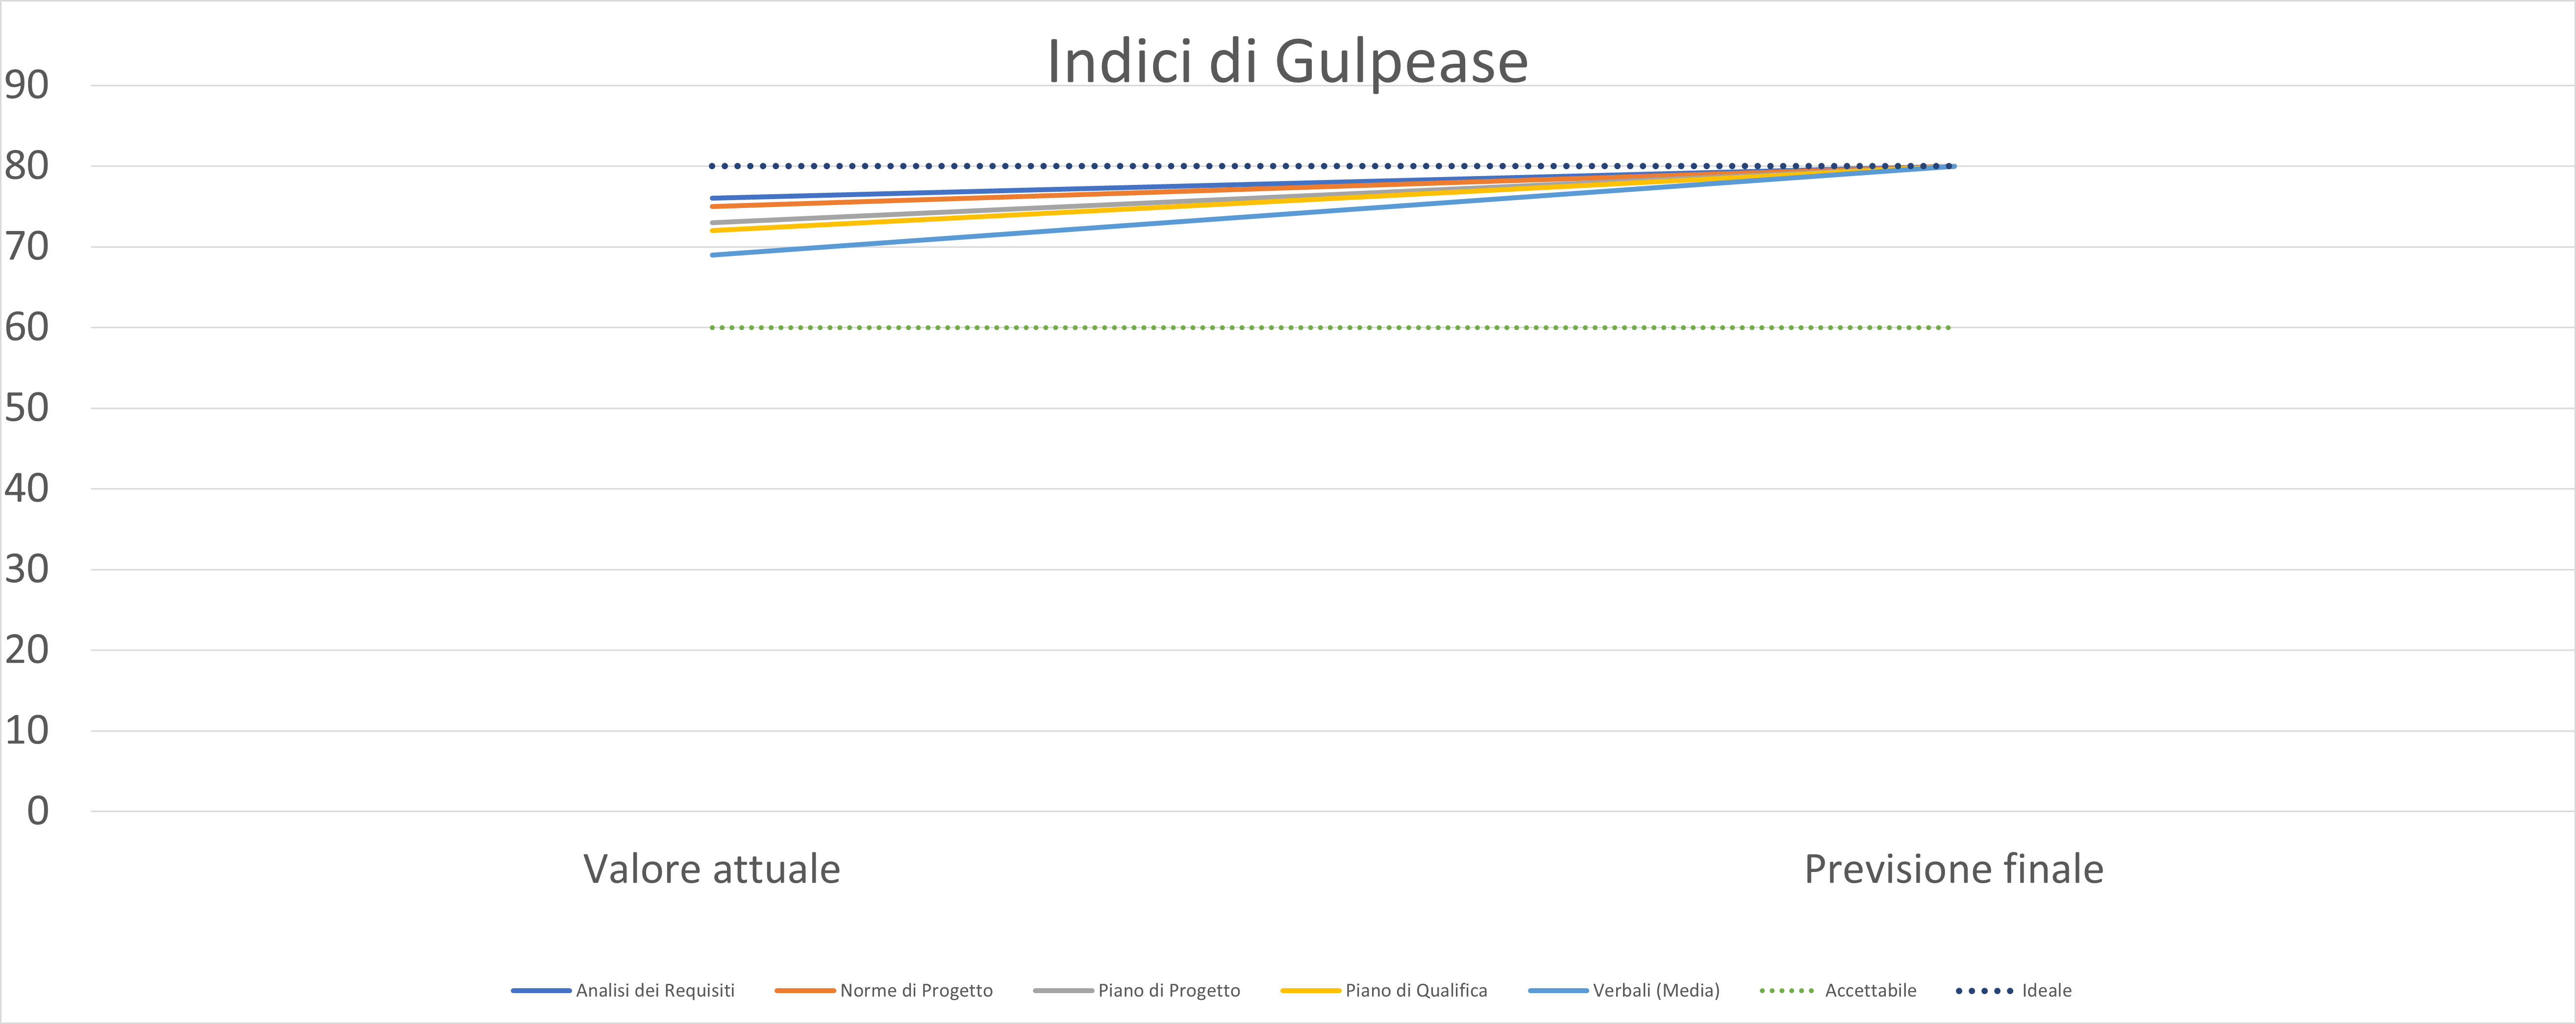
\includegraphics[width=\linewidth]{contenuti/img/gulpease.png}
    \caption{Indice Gulpease documentazione}
  \end{figure}

\section{Errori grammaticali}

\begin{center}
    \begin{xltabular}{\linewidth}{|l|l|l|}
    \hline
    \rowcolor[gray]{0.9}
    \textbf{Documento} & \textbf{Valore} & \textbf{Esito} \\
    \hline
     Analisi dei requisiti & 0 & Ideale \\
     Piano di qualifica & 0 & Ideale \\
     Piano di progetto & 0 & Ideale \\
     Norme di progetto & 0 & Ideale \\
     Verbali (media) & 0 & Ideale \\ 
    \hline

    \end{xltabular}
\end{center}

\chapter{Valutazioni per il miglioramento}\label{valutazioni-per-il-miglioramento}

\section{Valutazioni sull'organizzazione}
\begin{center}
    \begin{xltabular}{\linewidth}{|l|X|X|}
    \hline
    \rowcolor[gray]{0.9}
    \textbf{Attività} & \textbf{Problematica} & \textbf{Soluzione} \\
    \hline
     Incontri di gruppo & A causa dei diversi impegni di ciascun membro del gruppo, è risultato difficile in alcune settimane organizzare incontri, in particolare durante le prime settimane. & Si è deciso di effettuare riunioni regolari durante giorni generalmente liberi per tutti i membri, cercando compromessi su attività spostabili per ciascuno.\\
     Coordinazione dei lavori & A causa della mancanza di esperienza e della scostantezza sui lavori, ci siamo spesso trovati indietro sulla tabella di marcia. & % ?? % \\

    \hline

    \end{xltabular}
\end{center}

\section{Valutazioni sui ruoli}

\section{Valutazioni sugli strumenti di lavoro}

\begin{center}
    \begin{xltabular}{\linewidth}{|l|X|X|}
    \hline
    \rowcolor[gray]{0.9}
    \textbf{Strumento} & \textbf{Problematica} & \textbf{Soluzione} \\
    \hline
     GitHub & A causa della mancanza di esperienza di alcuni membri del gruppo, si sono riscontrati intoppi con l'utilizzo dello strumento, particolarmente nella fase iniziale del progetto. & I membri del gruppo con più esperienza hanno fornito aiuto a quelli con più carenze, in particolare spiegando come utilizzare il programma Fork per migliorare la sincronizzazione delle attività e semplificare l'uso della piattaforma. \\
     LaTeX & L'inesperienza di alcuni membri del gruppo ha causato alcune problematiche nella fase iniziale, in particolare sull'utilizzo di strutture più complesse come ad esempio tabelle. & I membri con meno esperienza hanno ricevuto aiuti da quelli con più conoscienza dello strumento, integrandoli con del tempo di studio individuale. \\

    \hline

    \end{xltabular}
\end{center}

\end{document}
